\chapter{Project}
%\label{chapter:title}
\section{The context}

The idea of processing in memory is an old one and has been considered since the mid 1990s~\cite{stone1970logic, Kautz1969, shaw1981non, kogge1994, gokhale1995processing, patterson1997case, oskin1998active, kang1999flexram, Mai:2000:SMM:339647.339673, Draper:2002:ADP:514191.514197,aga.hpca17,eckert2018neural,fujiki2019duality,kang.icassp14,seshadri.micro17,seshadri2013rowclone,angizi2019graphide,kim.hpca18,kim.hpca19,gao2020computedram,chang.hpca16,xin2020elp2im,li.micro17,deng.dac2018,hajinazarsimdram,rezaei2020nom,wang2020figaro,ali2019memory,li.dac16,angizi2018pima,angizi2018cmp,angizi2019dna,levy.microelec14,kvatinsky.tcasii14,shafiee2016isaac,kvatinsky.iccd11,kvatinsky.tvlsi14,gaillardon2016plim,bhattacharjee2017revamp,hamdioui2015memristor,xie2015fast,hamdioui2017myth,yu2018memristive,syncron,fernandez2020natsa,cali2020genasm,kim.bmc18,ahn.pei.isca15,ahn.tesseract.isca15,boroumand.asplos18,boroumand2019conda,singh2019napel,asghari-moghaddam.micro16,DBLP:conf/sigmod/BabarinsaI15,chi2016prime,farmahini2015nda,gao.pact15,DBLP:conf/hpca/GaoK16,gu.isca16,guo2014wondp,hashemi.isca16,cont-runahead,hsieh.isca16,kim.isca16,kim.sc17,DBLP:conf/IEEEpact/LeeSK15,liu-spaa17,morad.taco15,nai2017graphpim,pattnaik.pact16,pugsley2014ndc,zhang.hpdc14,zhu2013accelerating,DBLP:conf/isca/AkinFH15,gao2017tetris,drumond2017mondrian,dai2018graphh,zhang2018graphp,huang2020heterogeneous,zhuo2019graphq,santos2017operand,ghoseibm2019,wen2017rebooting,besta2021sisa,ferreira2021pluto,olgun2021quactrng,lloyd2015memory,elliott1999computational,zheng2016tcam,landgraf2021combining,rodrigues2016scattergather,lloyd2018dse,lloyd2017keyvalue,gokhale2015rearr,nair2015active,jacob2016compiling,sura2015data,nair2015evolution,balasubramonian2014near,xi2020memory}.
Despite being the first company to reach the stage of a commercially available PIM product, UPMEM is in need of technological demonstrators to encourage widespread adoption of its system.

My role during this apprenticeship was to develop machine-learning applications running on PIM that display an enticing performance gain (be it speed or energy consumption) when compared to existing CPU or GPU implementations.

\subsection{The technology}

\subsubsection{Motivation}

Data transfer on SDRAM is limited by a communication bus. Currently, the transfer rate on DDR5-6400 is 51.2 GB/s per channel (409.6 GB/s on an 8-channel system). Although this speed has been steadily increasing, there are popular algorithms today that end up with memory-bound performances (such as pooling operations in neural networks~\cite{nvidia.memory2020}).

The principle of PIM is to execute as many operations as possible in memory, and to minimize the number of operations that are executed in the CPU, thus limiting the flow of data through the memory bus.

\subsubsection{Architecture}

UPMEM DIMM is based on DDR4 and attaches an onboard RISC-V processor to each 64 MB memory bank, these processors are called DPU for Data Processing Units. A schematic representation of a DIMM can be seen in Figure \ref{fig:DIMM}. The transfer rate between each DPU and its associated memory bank is 1 GB/s. This means that on a server with the maximum number of DPUs (2560), the total transfer rate is 2.5 TB/s.

\begin{figure}[htb]
    \centering
    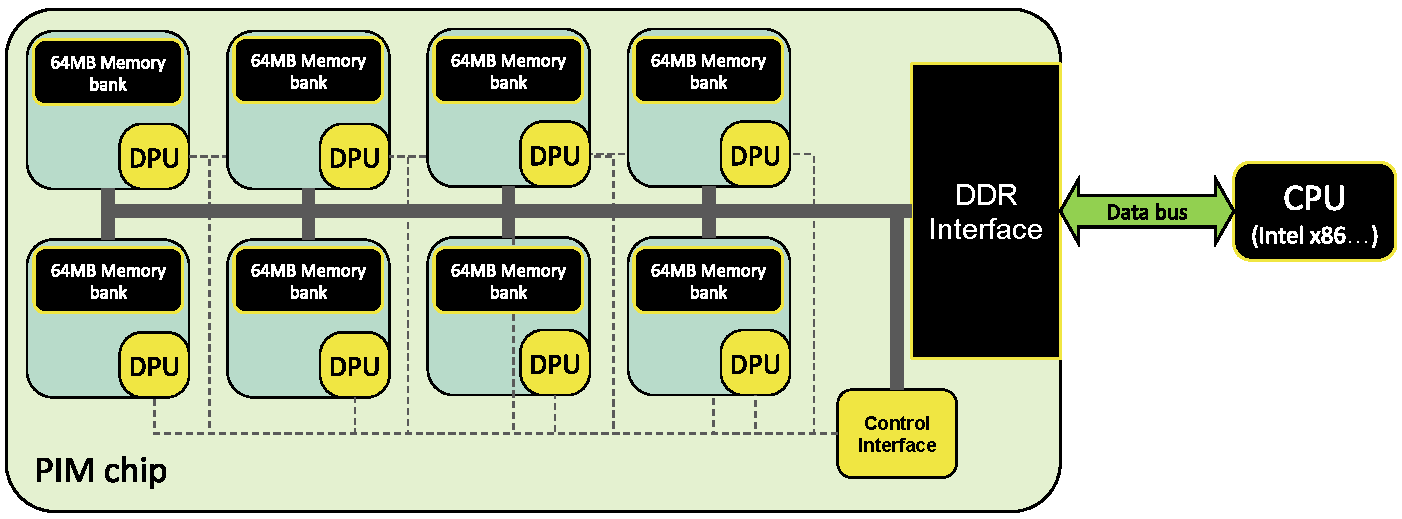
\includegraphics[width=0.95\linewidth]{figures/PIM.pdf}
    \caption{\label{fig:DIMM}UPMEM PIM Architecture}
\end{figure}

Each DIMM has two ranks with 64 DPUs each. This amounts to 8.2 GB of memory per DIMM.

